\documentclass{article}

\title{Chapter 1: Real Numbers and Functions}
\author{}
\date{}

\usepackage[left=3.5cm, right=3.5cm]{geometry}
\usepackage{tikz}
\usepackage{amsmath}
\usepackage{amssymb}
\usepackage{outlines}
\usepackage[most]{tcolorbox}
\usepackage{setspace}
\usepackage{tabularx,colortbl}
\usepackage[dvipsnames]{xcolor}
\usetikzlibrary{arrows}

\definecolor{myblue}{RGB}{122, 216, 235}
\colorlet{babyblue}{myblue!30}

\newcommand{\tb}[1]{\textbf{#1}}
\newcommand{\ul}[1]{\underline{#1}}
\newenvironment{mybox}[3]{
    \begin{center}
    \begin{tcolorbox}[width=#2\textwidth, colback={#3}, colbacktitle={#3}, title={\tb{#1}}, coltitle={black}, colframe={#3}, arc=1pt, breakable]}
    {\end{tcolorbox} 
    \end{center}}

\begin{document}

\maketitle

\section{The Real Line and Inequalities}

\subsection{Real Numbers}

The real numbers can be visualized using a coordinate system known as the \textbf{real line}. Every number on this line corresponds to some real number.

\begin{center}
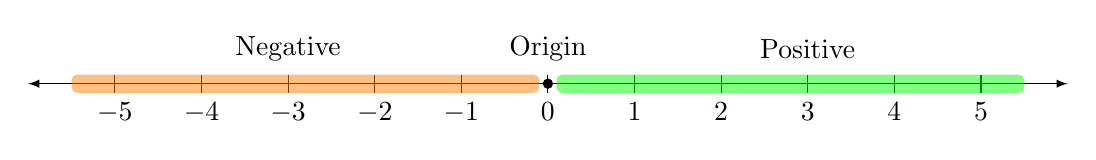
\begin{tikzpicture}[scale=1.1]
\draw[latex-latex] (-6,0) -- (6,0) ; %edit here for the axis
\foreach \x in  {-5,-4,-3,-2,-1,0,1,2,3,4,5} % edit here for the vertical lines
\draw[shift={(\x,0)},color=black] (0pt,3pt) -- (0pt,-3pt);
\foreach \x in {-5,-4,-3,-2,-1,0,1,2,3,4,5} % edit here for the numbers
\draw[shift={(\x,0)},color=black] (0pt,0pt) -- (0pt,-3pt) node[below] 
{$\x$};
\draw[opacity=0, fill=orange, fill opacity=0.5, rounded corners=2pt] (-0.1, 3pt) rectangle (-5.5, -3pt);
\draw[opacity=0, fill=green, fill opacity=0.5, rounded corners=2pt] (0.1, 3pt) rectangle (5.5, -3pt);
\node[] at (-3, 0.4) {Negative};
\node[] at (3, 0.4) {Positive};
\node[] at (0, 0.4) {Origin};
\draw[fill=black] (0,0) circle (1.5pt);

\end{tikzpicture}
\end{center}

The point on the real line corresponding to zero is called the \textbf{origin}. All of the numbers to the right of the origin (in green) are \textbf{positive} and numbers to the left of the origin (in orange) are \textbf{negative}. We also use the terms \textbf{nonnegative} (resp.~\textbf{nonpositive}) to refer to the positive numbers and $0$ (resp.~negative numbers and 0).

\vspace{5pt}
The following are a list of important sets of real numbers to know along with symbols commonly used to denote them.

\begin{outline}
    \1 \tb{Natural Numbers} ($\mathbb{N}$): $\{1, 2, \ldots\}$ These are the counting numbers, the ones you grew up learning. Sometimes $0$ is also considered to be a natural number, though I will not do so in this class (unless stated otherwise).
    \1 \tb{Integers} ($\mathbb{Z}$): $\{\ldots, -2, -1, 0, 1, 2, \ldots\}$ These are all of the counting numbers and their negatives. Everything in this set still has ``whole-number values'', so it does \emph{not} include things like $\frac{1}{4}$ and $0.333 \ldots$
    \1 \tb{Rational Numbers} ($\mathbb{Q}$): $\{\frac{a}{b}\,|\, a \textrm{ and } b \textrm{ are integers and } b \neq 0\}$ The rational numbers include all fractions and repeating decimals, so things like $\frac{2}{3}, \frac{7}{5},$ and $4.111\ldots$ are included in this set. It is important to note that the rational numbers also include the integers, since for example $3$ can be written as $\frac{3}{1}$ or $\frac{6}{2}$.
    \1 \tb{Irrational Numbers}: The irrational numbers are all numbers which aren't rational. Some notable examples include $\sqrt{2}, \pi$, and $e$. One can tell these are all indeed irrational numbers since their decimal expansions do not repeat:
        \2 $\sqrt{2} = 1.414213562 \ldots$
        \2 $\pi = 3.14592654 \ldots$
        \2 $e = 2.718281828 \ldots$
    \1[] From here, it looks like $e$ repeats, but you can find more digits to show it does not. The irrational numbers don't have a special symbol.
\end{outline}

\subsection{Inequalities and Intervals}

Since all of the real numbers can be arranged from left-to-right, we call them \tb{ordered}. The following is some terminology related to the ordering on the real line.

\vspace{5pt}
\begin{outline}
    \0 Let $x$ and $y$ denote real numbers, then:
    \1 We say $x$ is \tb{less than} $y$ (denoted $x<y$) if $x$ lies to the \emph{left} of $y$ on the real line.
    \1 We say $x$ is \tb{greater than} $y$ (denoted $x>y$) when $x$ is to the \emph{right} of $y$ on the real line.
    \1 We say $x$ is \tb{less than or equal to} $y$ if $x<y$ or $x=y$.
    \1 We say $x$ is \tb{greater than or equal to} $y$ if $x>y$ or $x=y$.
\end{outline}

Sometimes the inequalities $x<y$ and $x>y$ are referred to as \emph{strict inequalities} since the two numbers $x$ and $y$ are not allowed to be equal. It will be important in this course to be able to manipulate/perform algebra on inequalities. For this reason, we now introduce several important properties of inequalities.

\begin{mybox}{Properties of Inequalities}{0.8}{babyblue}
    \doublespacing
    Let $a,b,c,d$ and $k$ be real numbers.

    \indent \quad (Symmetric) $a<b$ if and only if $b>a$. \\ 
    \indent \quad (Transitive) If $a<b$ and $b<c$, then $a<c$. \\ 
    \indent \quad (Adding Constants) If $a<b$, then $a+k<b+k$. \\
    \indent \quad (Adding Inequalities) If $a<b$ and $c<d$, then $a+c<b+d$. \\
    \indent \quad (Positive Multiplication) If $a<b$ and $k$ is positive, then $ak < bk$. \\
    \indent \quad (Negative Multiplication) If $a<b$ and $k$ is negative, then $ak > bk$
\end{mybox}

A few remarks about these properties: All of the above properties are true if $<$ or $>$ is replaced with $\leq$ or $\geq$ respectively. Similarly, all of the above properties are true for equations ($=$) as well, ignoring the need to ``flip'' signs when multipliying.

\vspace{5pt}
Inequalities are particularly useful in describing sets of numbers on the real line. For example, the positive numbers are all of the numbers $x$ where $x>0$. Similarly, the negative numbers are those numbers $x$ which satisfy $x<0$. At the moment, this is a very wordy way of describing sets of numbers. To fix this, we introduce \tb{set notation}.

\begin{mybox}{Set Notation}{0.9}{babyblue}
    To define a set of real numbers, the \emph{set notation} $\{x \,|\, \textrm{condition on }x \}$ denotes all of the real numbers $x$ which satisfy the given condition. These are a few common sets of numbers written in set notation:

    \vspace{5pt}
    \begin{itemize}
        \setlength\itemsep{0em}
        \item Positive Numbers: $\{x \,|\, x>0\}$
        \item Negative Numbers: $\{x \,|\, x<0\}$
        \item Even Numbers: $\{x \,|\, x=2k \textrm{ where } k \textrm{ is an integer}\}$
        \item Odd Numbers: $\{x \,|\, x=2k + 1 \textrm{ where } k \textrm{ is an integer}\}$
        \item Powers of 2: $\{x \,|\, x=2^k \textrm{ where } k \textrm{ is an natural number}\}$
    \end{itemize}
\end{mybox}

While real numbers are commonly denoted with lowercase letters like $x,y,z$, sets are denoted with capital letters like $A$ and $B$. Commonly-used sets like the integers and rational numbers are given bolded letters like $\mathbb{Z}$ and $\mathbb{Q}$ to denote their importance. The following is some important terminology involving sets.

\vspace{5pt}
\begin{outline}
    \0 Let $x$ be a real number and $A, B$ be sets of real numbers, then:
    \1 When $x$ is \tb{contained in} the set $A$, we write $x \in A$. Similarly if $x$ is \tb{not contained in} $A$, we write $x \not\in A$. 
    \1 $A \cup B = \{x \,|\,x\in A \textrm{ or } x \in B\}$ is the \tb{union} of $A$ and $B$, and it consists of all of the numbers in either $A$, $B$, or both.
    \1 $A \cap B = \{x \,|\,x\in A \textrm{ and } x \in B\}$ is the \tb{intersection} of $A$ and $B$, and it consists of all of the numbers in both $A$ and $B$.
    \1 We say the sets $A$ and $B$ are \tb{disjoint} if they have no elements in common (i.e. $A \cap B$ is empty).
\end{outline}

One important class of sets used frequently in calculus are \tb{intervals} - visually, these are the sets which look ``connected''. Below is a table of different types intervals.

\vspace{5pt}

\begin{mybox}{Types of Intervals}{0.9}{babyblue}

Let $a$ and $b$ be real numbers where $a<b$, then the following are all different types of intervals on the real line.
\vspace{5pt}

% Open Interval
\ul{Open Interval:} {\large \qquad $(a,b) = \{x \,|\, a < x < b\}$}

\vspace{10pt}

\begin{center}
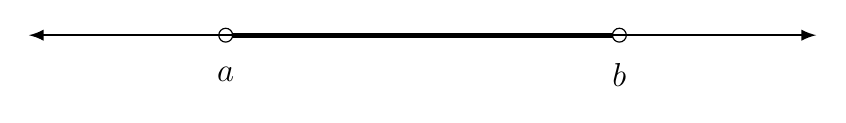
\begin{tikzpicture}[scale=2.5]
    \draw[line width=0.6mm] (-1,0) -- (1,0);
    \draw[line width=0.15mm, fill=white] (-1,0) circle (1pt);
    \draw[line width=0.15mm, fill=white] (1,0) circle (1pt);
    \node[] at (-1,-0.2) {\large$a$};
    \node[] at (1,-0.2) {\large$b$};
    \draw[latex-latex, line width=0.3mm] (-2,0) -- (2,0); % edit here for the axis
    
\end{tikzpicture}
\end{center}

% Closed Interval
\ul{Closed Interval:} {\large \qquad $[a,b] = \{x \,|\, a \leq x \leq b\}$}
\vspace{10pt}
\begin{center}
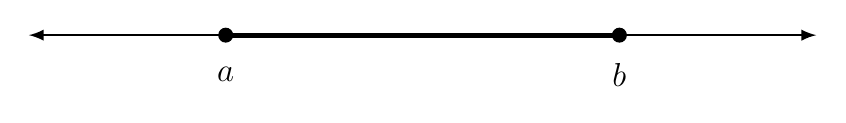
\begin{tikzpicture}[scale=2.5]
    \draw[line width=0.6mm] (-1,0) -- (1,0);
    \draw[fill=black] (-1,0) circle (1pt);
    \draw[fill=black] (1,0) circle (1pt);
    \node[] at (-1,-0.2) {\large$a$};
    \node[] at (1,-0.2) {\large$b$};
    \draw[latex-latex, line width=0.3mm] (-2,0) -- (2,0); % edit here for the axis
    
\end{tikzpicture}
\end{center}

\vspace{20pt}

% Half-Open Interval 1
\ul{Half-Open Intervals:} {\large \qquad $[a,b) = \{x \,|\, a \leq x < b\}$}
\vspace{10pt}
\begin{center}
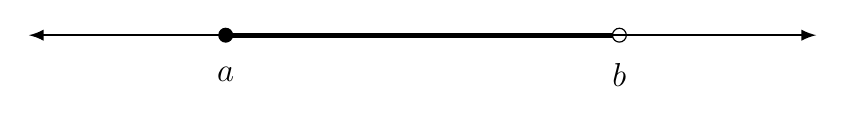
\begin{tikzpicture}[scale=2.5]
    \draw[line width=0.6mm] (-1,0) -- (1,0);
    \draw[fill=black] (-1,0) circle (1pt);
    \draw[line width=0.15mm, fill=white] (1,0) circle (1pt);
    \node[] at (-1,-0.2) {\large$a$};
    \node[] at (1,-0.2) {\large$b$};
    \draw[latex-latex, line width=0.3mm] (-2,0) -- (2,0); % edit here for the axis
    
\end{tikzpicture}
\end{center}

% Half-Open Interval 2
\begin{center}{\large \quad $(a,b] = \{x \,|\, a < x \leq b\}$}\end{center}
\begin{center}
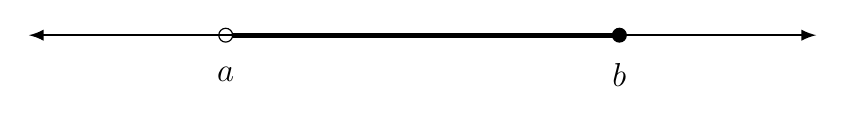
\begin{tikzpicture}[scale=2.5]
    \draw[line width=0.6mm] (-1,0) -- (1,0);
    \draw[fill=black] (1,0) circle (1pt);
    \draw[line width=0.15mm, fill=white] (-1,0) circle (1pt);
    \node[] at (-1,-0.2) {\large$a$};
    \node[] at (1,-0.2) {\large$b$};
    \draw[latex-latex, line width=0.3mm] (-2,0) -- (2,0); % edit here for the axis
    
\end{tikzpicture}
\end{center}

% Open Rays
\ul{Open Rays:} {\large \qquad \qquad \quad $(-\infty,b) = \{x \,|\, x < b\}$}
\begin{center}
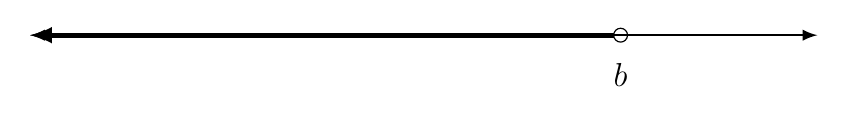
\begin{tikzpicture}[scale=2.5]
    \draw[latex-, line width=0.6mm] (-2,0) -- (1,0);
    \draw[line width=0.15mm, fill=white] (1,0) circle (1pt);
    \node[] at (1,-0.2) {\large$b$};
    \draw[latex-latex, line width=0.3mm] (-2,0) -- (2,0); % edit here for the axis
    
\end{tikzpicture}
\end{center}

\begin{center}{\large $(a,\infty) = \{x \,|\, a < x \}$}\end{center}
\begin{center}
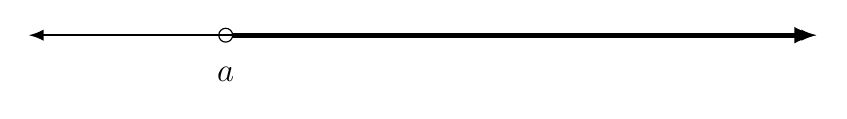
\begin{tikzpicture}[scale=2.5]
    \draw[latex-, line width=0.6mm] (2,0) -- (-1,0);
    \draw[line width=0.15mm, fill=white] (-1,0) circle (1pt);
    \node[] at (-1,-0.2) {\large$a$};
    \draw[latex-latex, line width=0.3mm] (-2,0) -- (2,0); % edit here for the axis
    
\end{tikzpicture}
\end{center}


% Closed Rays
\ul{Closed Rays:} {\large \qquad \qquad \quad $(-\infty,b] = \{x \,|\, x \leq b\}$}
\begin{center}
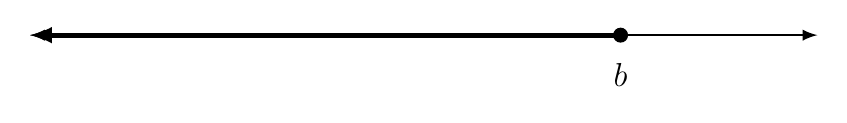
\begin{tikzpicture}[scale=2.5]
    \draw[latex-, line width=0.6mm] (-2,0) -- (1,0);
    \draw[fill=black] (1,0) circle (1pt);
    \node[] at (1,-0.2) {\large$b$};
    \draw[latex-latex, line width=0.3mm] (-2,0) -- (2,0); % edit here for the axis
    
\end{tikzpicture}
\end{center}

\begin{center}{\large $[a,\infty) = \{x \,|\, a \leq x \}$}\end{center}
\begin{center}
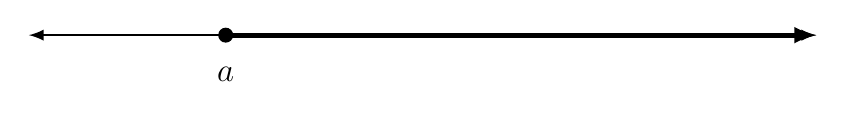
\begin{tikzpicture}[scale=2.5]
    \draw[latex-, line width=0.6mm] (2,0) -- (-1,0);
    \draw[fill=black] (-1,0) circle (1pt);
    \node[] at (-1,-0.2) {\large$a$};
    \draw[latex-latex, line width=0.3mm] (-2,0) -- (2,0); % edit here for the axis
    
\end{tikzpicture}
\end{center}

% All Real Numbers
\ul{All Real Numbers:} {\large \qquad \qquad $(-\infty,\infty)$}
\begin{center}
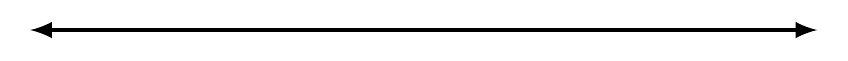
\begin{tikzpicture}[scale=2.5]
    \draw[latex-latex, line width=0.6mm] (-2,0) -- (2,0); % edit here for the axis
    
\end{tikzpicture}
\end{center}

\end{mybox}

Interval notation is central to many of the problems at the heart of calculus. Solutions to inequalities, increasing/decreasing intervals for functions and domain restrictions are just a few applications which will come up this semester, so being comfortable with this sort of notation is important.

\section{The Cartesian Coordinate System}


\section{Graphing Equations}


\section{Lines in the Plane}


\section{Functions}

\end{document}